\documentclass[12pt,twoside,onecolumn]{article}

\usepackage{a4}
\usepackage[dvipsnames]{xcolor}
\usepackage[margin=0.75in]{geometry}
\usepackage{pdfpages}
\usepackage{apacite}
\usepackage{jneurosci}
\usepackage[utf8]{inputenc}
\usepackage[T1]{fontenc}
\usepackage[norsk]{babel}
\usepackage{subfiles} % Handeling multiple chapters on seperate files.
\usepackage{graphicx}  % for displaying figures
\usepackage{subcaption}
\usepackage{url}
\usepackage{amsmath} % math package
\usepackage{relsize} % to use larger math symbols
\usepackage{amssymb} % for using blackboard letters (e.g R for real numbers)
\usepackage{tocbibind} % for adding the reference section in table of contents
%\usepackage{fixltx2e} % for text in sub script
\usepackage{perpage} % for resetting footnote counter at each page
\usepackage{csquotes}
\usepackage{epigraph}
\usepackage{ragged2e}
\usepackage{exercise}
\usepackage{amsmath}
\usepackage{soul}


\MakePerPage{footnote} %the perpage package command

\addto\captionsenglish{%
  \renewcommand{\figurename}{Figur}
}

\addto\captionsenglish{\renewcommand{\exercisename}{Oppgave}}

\makeatletter
\def\@documentnocite#1{\@bsphack
  \@for\@citeb:=#1\do{%
    \edef\@citeb{\expandafter\@firstofone\@citeb}%
    \if@filesw\immediate\write\@auxout{\string\citation{\@citeb}}\fi
    \@ifundefined{b@\@citeb}{\G@refundefinedtrue
      \@latex@warning{Citation `\@citeb' undefined}}{}}%
  \@esphack}
\AtBeginDocument{\let\nocite\@documentnocite}
\makeatother

\begin{document}

\hspace{-6mm}Denne skriften er det brukeren ser, inkludert skrift som er fargelagt {\color{red}rødt} og {\color{blue}blått}\newline
{\color{gray} Skriften brukes til å refere til manus} \newline
{\color{PineGreen} Skriften brukes til å refere til videodesign} \newline
{\color{Maroon} Skriften brukes til å refere til handlinger i plattformen} \newline
{\color{Cerulean} Skriften brukes til å stille design spørsmål}

\section*{Ligninger}

\subsection*{Førstegradsligninger}

\begin{Exercise}
\begin{align}
7x - 3 &= 11  \qquad\text{ Plus 3 på begge sider av likhetstegnet.}\\
7x -3 +3 &= 11 + 3\\
7x &= 14\\  
\frac{7x}{7} &=  \frac{14}{7} \qquad\text{ Uttrykket kan forkenkles mer.}\\
x &= 2
\end{align}
\end{Exercise}

\begin{Exercise}
\textbf{Del 1}
\begin{align}
\frac{x}{2} + \frac{5}{6} &=  \frac{4}{3} - x \qquad\text{ Pluss x på begge sider av likhetstegnet.}\\
\frac{x}{2} + x + \frac{5}{6} &=  \frac{4}{3} - x + x\\
\frac{x}{2} + x + \frac{5}{6} - \frac{5}{6} &=  \frac{4}{3} - \frac{5}{6}\\
\frac{x}{2} + \frac{2x}{2} &= \frac{8}{6} - \frac{5}{6}\\
\frac{3x}{2}  &= \frac{3}{6} \qquad\text{ Uttrykket kan forkenkles mer.}\\ 
\frac{3x\cdot2}{7\cdot3} &=  \frac{1\cdot2}{2\cdot3} \qquad\text{ Uttrykket kan forkenkles mer.}\\
x &= \frac{1}{2}
\end{align}
\end{Exercise}

\subsection*{Sett inn tall i ligninger}
\begin{Exercise}
Fatima har kjøpt nytt abonnement hos Telixor. I abonnementet har hun en fast beløp hver måned på 50 kr. I tillegg må hun betale 1.50 kr per MB hun bruker. 
\newline\newline
\textbf{Del 1)} Lag en ligning som beskriver Fatimas total månedlig kostnad. La x være antall MB hun bruker i måneden og P(x) hennes total kostnad per måned.
\begin{align}
P &= 50 \text{ Hvis Fatima bruker ingen data, blir da hennes forbruk lik 50}\\ 
P &= 50 + 1.5\cdot1\text{ Hvis Fatima bruker 1MB data, blir da hennes forbruk lik $50 + 1.5\cdot1$}\\ 
P &= 50 + 1.5\cdot2\text{ Hvis Fatima bruker 2MB data, blir da hennes forbruk lik $50 + 1.5\cdot2$}\\ 
&\text{ Hva blir hennes forbruk hvis hun bruker x-antall data per måned} \nonumber\\
P &= 50 + 1.5x
\end{align}
\newline
\textbf{Del 2)}
Finn hennes total kostnad per måned når hun bruker 1000 MB = 1 GB data.
\begin{align}
P &= 50 + 1.5\cdot1000\\
P &= 50 + 1500\\
P &= 1550
\end{align}
Vil du si at dette er et bra abonnement for Fatima i år 2017 ?
\end{Exercise}

\section*{Funksjoner}

\begin{Exercise}
Vennligst klikk følgende koordinat i planet:$(0,1)$
\begin{figure}[h!]
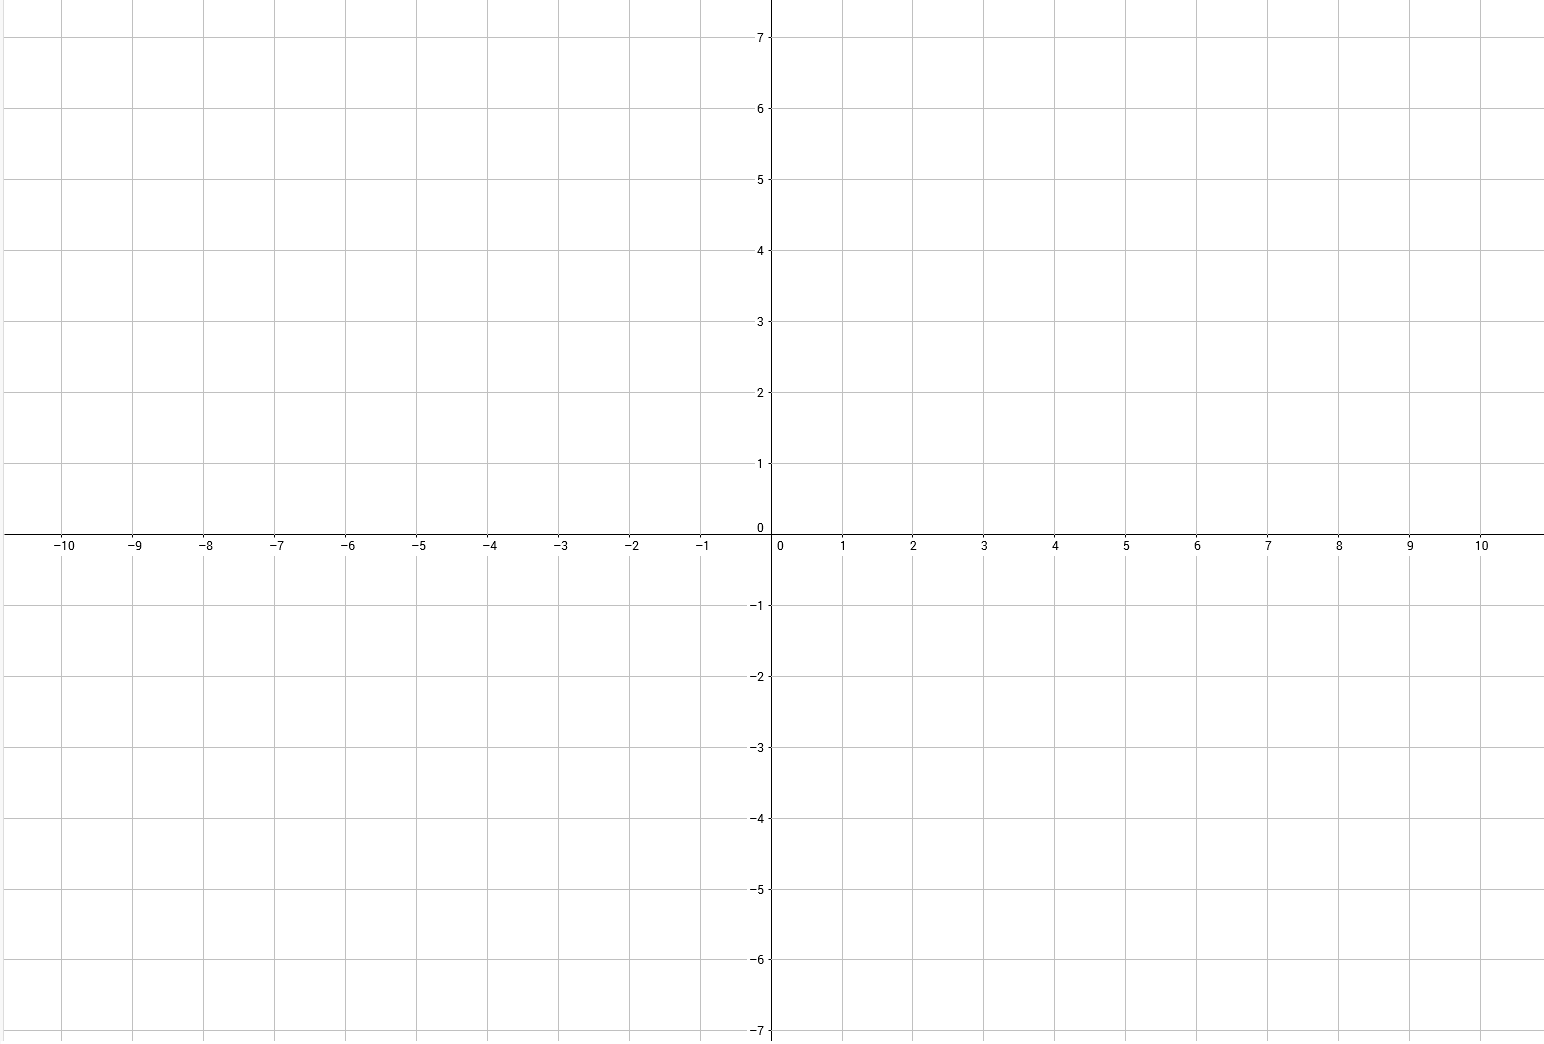
\includegraphics[scale = 0.3]{figures/Grid.png}
\label{fig:grid}
\end{figure}
\newline
{\color{Maroon}Hvis bruker taster feil, får han lov til en ny sjanse}
\newline
Vennligst klikk følgende koordinat i planet: $(3,1)$
\newline
{\color{Maroon}Hvis bruker taster feil denne gangen vil han få en hint - hint knappen blir synlig}
\newline\newline
\textbf{Hint:}  $(x,y) = (3,1)$, dvs. at $x = 3$ og $y = 1$. Prøv å vis dette punktet i planet.
\newline
\newline
{\color{Maroon}Hvis bruker taster feil på flere slike oppgaver vil han få en video med forklaring :} 
\newline
La oss se på punkt (4,2) og (-3,5). Vi vil nå vise at disse punktene ligger henholdsvis i første og andre kvadrant.
Husk at den horisontale koordinat aksen (x-aksen) er alltid den første koordinat ({\color{PineGreen}På videoen blir et punktene hevet med grafikk}), mens det andre tallet i tall paret er langs den vertikale koordinat aksen (y-aksen).
\newline
\newline
{\color{Maroon}Hvis bruker taster riktig på flere slike oppgaver vil han gå videre til neste oppgave.}
\end{Exercise}

\begin{Exercise}
Følgende ligning beskriver en lineær funksjon:
\begin{align}
y = 3x + 2.
\end{align}
Hva er y verdien når $x = 2$. \newline
{\color{Maroon} Hvis bruker taster feil, får hun følgende hint.} \newline
\textbf{Hint:} Du må erstatte x variablen med verdien 2. \newline\newline
{\color{Maroon} Hvis eleven oppgir feil y verdi vil han få riktig svar fylt vha. en animasjon.}\newline
{\color{Cerulean} Hvordan bør animasjonen lages?} \newline
{\color{Maroon} Hvis eleven bruker hint, får han en ny oppgave med en annen tallverdi.}
\end{Exercise}

\begin{Exercise}
\textbf{Del 1} \newline
En funksjon er gitt ved $y = -2x + 1$. Du skal fylle verdiene i tabellen under.
\begin{center}
    \begin{tabular}{ | l | l | p{3cm} |}
    \hline
    x  &  y  &  \\ \hline
    0  &     & {\color{Maroon} $y = -2\cdot \underline{\phantom{x}}  + 1$} \\ \hline
    3  &     & {\color{Maroon} $y = -2\cdot \underline{\phantom{x}}  + 1$} \\ \hline
    -2 &     & {\color{Maroon} $y = -2\cdot \underline{\phantom{x}}  + 1$} \\ \hline
	   & -7  & {\color{Maroon} $\underline{\phantom{y}} = -2\cdot x  + 1$} \\ \hline
	   &  1   & {\color{Maroon} $\underline{\phantom{y}} = -2\cdot x  + 1$} \\ \hline	   
    \end{tabular}
\end{center}
{\color{Maroon} De siste to verdiene er kun ment for sterke elever og vil ikke være synlig for svake elever.}\newline 
{\color{Cerulean} Tredje kolonne oppstår når eleven vet ikke hva eller hvordan hun skal finne verdiene. Eleven vil da veiledes interaktivt, med for eksempel en pil over hvor tall verdien skal og hvilken tall verdi.}
\newline
\newline
Hvis eleven trenger video forklaring, får han følgende løsningsforlag/demonstrasjon.
\begin{enumerate}
\item {\color{PineGreen}Videoen startet med tabellen}
    \begin{tabular}{ | l | l |}
    \hline
    x  &  y  \\ \hline
    0  &     \\ \hline
    3  &   \\ \hline
    -2 &   \\ \hline
	\end{tabular}
\item {\color{Maroon}Vi har gitt en lineær funksjon og målet til oppgaven er å finne y verdiene for de gitte x verdiene i tabellen. Det vil si, vi må sette hver x verdi inn i funksjonen og regne ut y verdien.}\\
{\color{PineGreen}Skriver ut funksjonen ved siden av tabellen og indikerer variablen x som skal erstattes.}
\item {\color{PineGreen}Mens det skrives ned utregning for hver y, skal oppleser lese av operasjonene.}
\end{enumerate}

\textbf{Del 2} \newline
I denne oppgaven skal du sette tall parene for x og y koordinatene inn i planet for å visualisere grafen.\newline
{\color{Cerulean}Hvis bruker har tastet punktene i riktig koordinater, vil elven få oppgaven godkjent. Det vises en funksjon som går gjennom punktene.} \newline
{\color{Maroon}Hvis eleven blander x med y koordinater, vil han få hint om å passe på rekkefølgen når leser av på koordinataksene.}\newline
{\color{Cerulean}Hvis bruker taster inn koordinater på feil sted, vil hans punkter bli sammenlignet med riktig punkter.}\newline{\color{Cerulean}Hvis bruker taster riktig eller feil skal han få en eller annen tilbakemelding når han taster inn hver tall verdi i tabellen.}
{\color{Cerulean}Hvis bruker taster riktig eller feil skal han få en eller annen tilbakemelding når han taster inn hver tall verdi i tabellen.}
\newline\newline
Hvis bruker ber om video forklaring får han følgende løsning/demonstrasjon:
\begin{enumerate}
\item {\color{Gray}Nå skal vi sett disse punktene i planet.} \newline
\begin{figure}[h!]
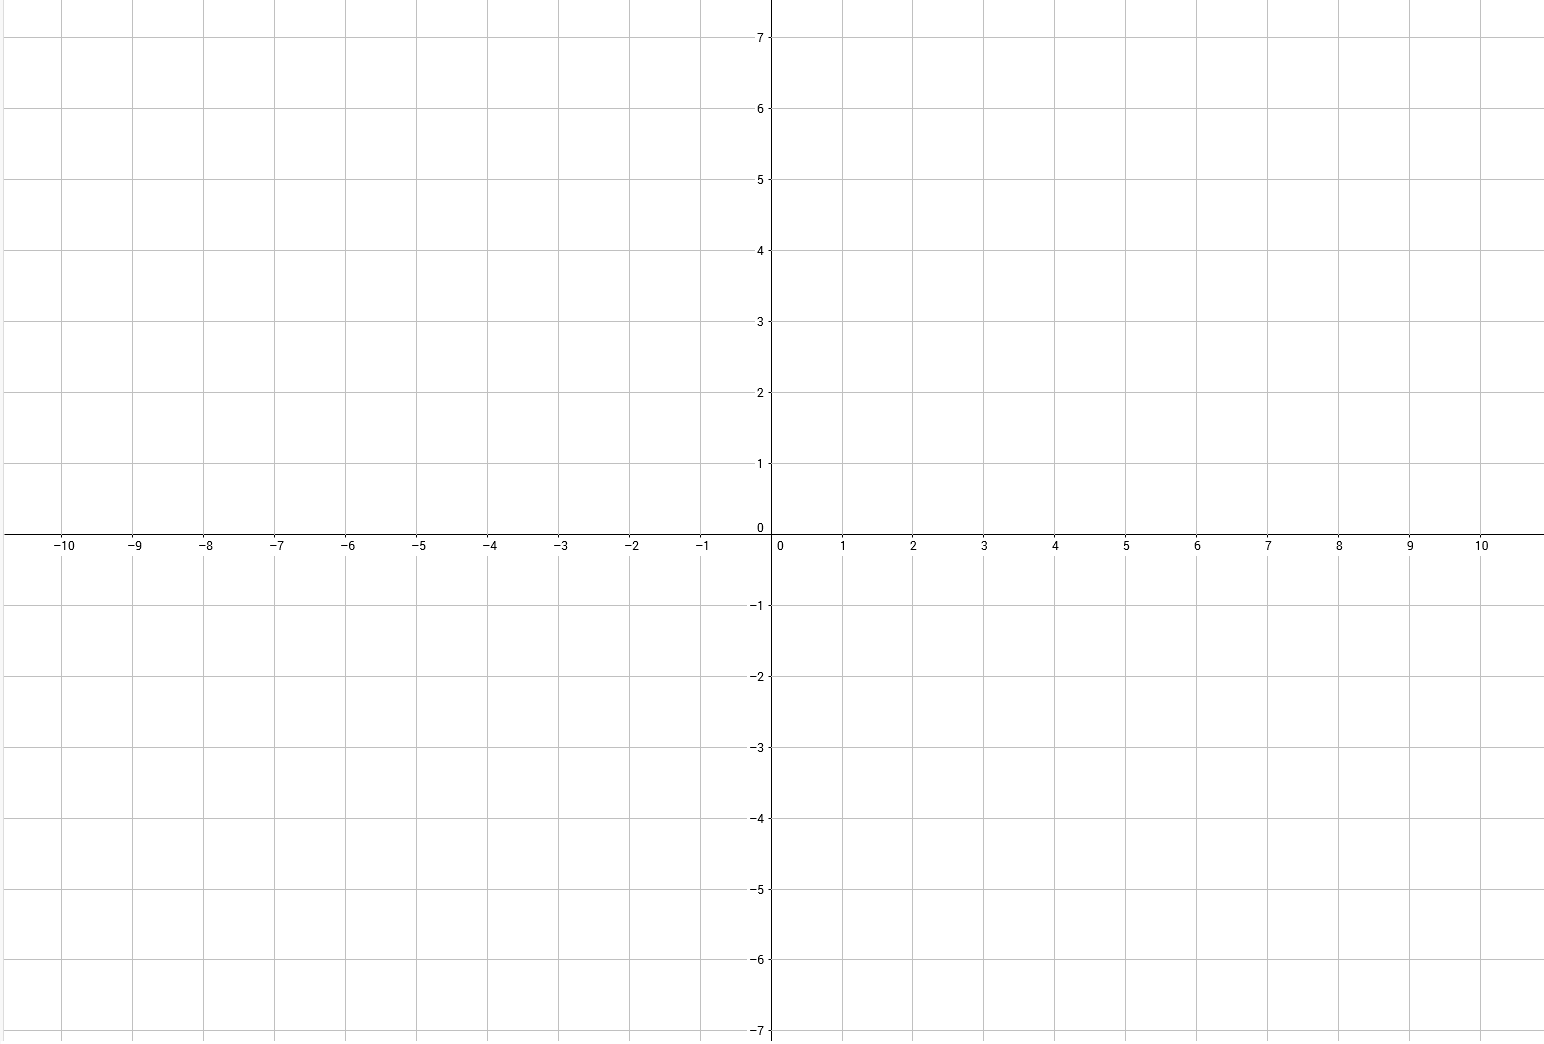
\includegraphics[scale = 0.1]{figures/Grid.png}
\end{figure}
{\color{PineGreen} Videoen starter med grid og punktene blir utpekt og demonstrert når oppleser leser av instruksjonen.}
\item {\color{Gray}For eksempel, la oss begynne med punkt (3,-5). Vi skal bevege oss fra origo 3 plasser langs x-aksen mot høyre ..... og videre beveger vi oss 5 plasser ned fra x-aksen i 4 kvadrant,  dvs. under x-aksen til høyre.}
\item {\color{Gray}Punkt (-2,5) vi beveger oss 2 plasser horizontalt til venstre og 5 plasser vertikalt i 2 kvadrant (over x-aksen til venstre).}
\item {\color{Gray}Punkt (0,1) er 0 i x koordinaten og 1 i y koordinaten. For å plassere punktet holder vi oss langs y aksen, siden $x=0$ og flytter 1 plass vertikalt.}
\end{enumerate}
\end{Exercise}

%%%%%%%%%%%%%%%%%%%%%%  Stigningstallet %%%%%%%%%%%%%%%%%%%
\subsection*{Stigningstallet}

\begin{Exercise}
Finn stignigstallet til følgende lineære funksjoner. Fyll svaret i svarfeltet :
\begin{figure}[h!]
\centering

\includegraphics[scale = 0.3]{figures/Svarfelt.png}
\label{fig:grid}
\end{figure}
{\color{Maroon}Hvis eleven taster feil:} Husk at stigningstallet beskriver hvor mye funksjonen vokser eller minker når du øker x verdien. Husk at stigningstallet er gitt som forandring i y-verdien delt på forandringen i x-verdien:
\begin{align}
a = \frac{\Delta y}{\Delta x} = \frac{y_2 - y_1}{x_2 - x_1}
\end{align}
\begin{figure}[h!]
\centering
    \begin{subfigure}{.5\textwidth}
    \centering
    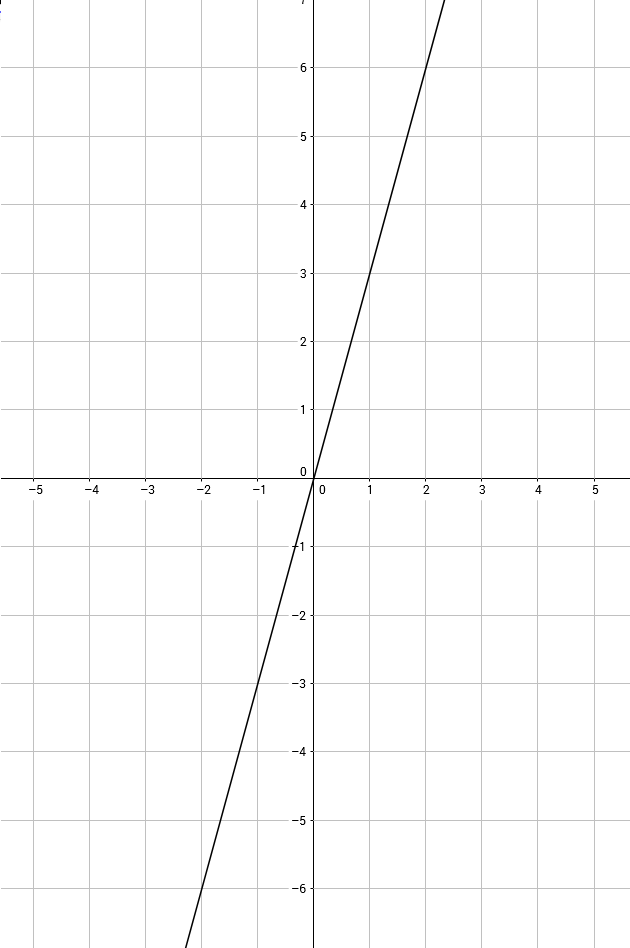
\includegraphics[scale = 0.5]{figures/3X.png}
    \end{subfigure}%%
    \begin{subfigure}{.5\textwidth}
    \centering
    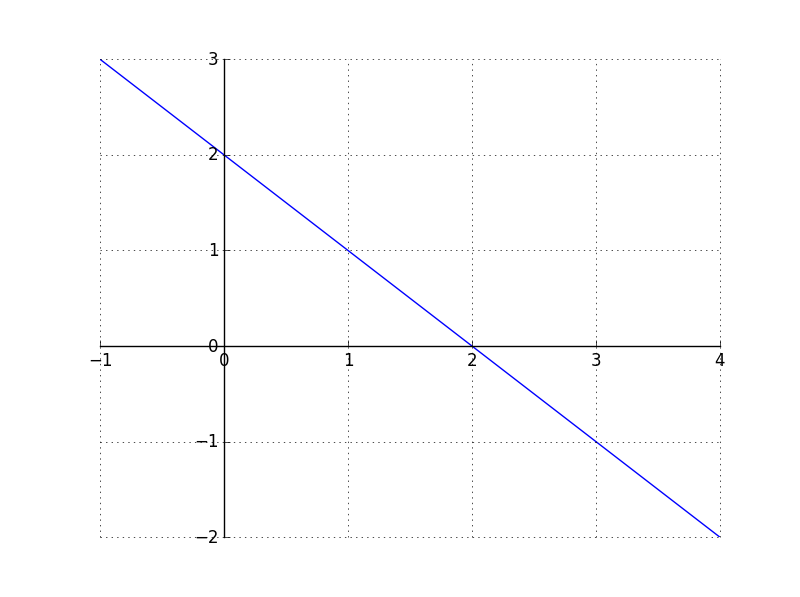
\includegraphics[scale = 0.5]{figures/mXp2.png}
    \end{subfigure}
    \begin{subfigure}{.5\textwidth}
    \centering
    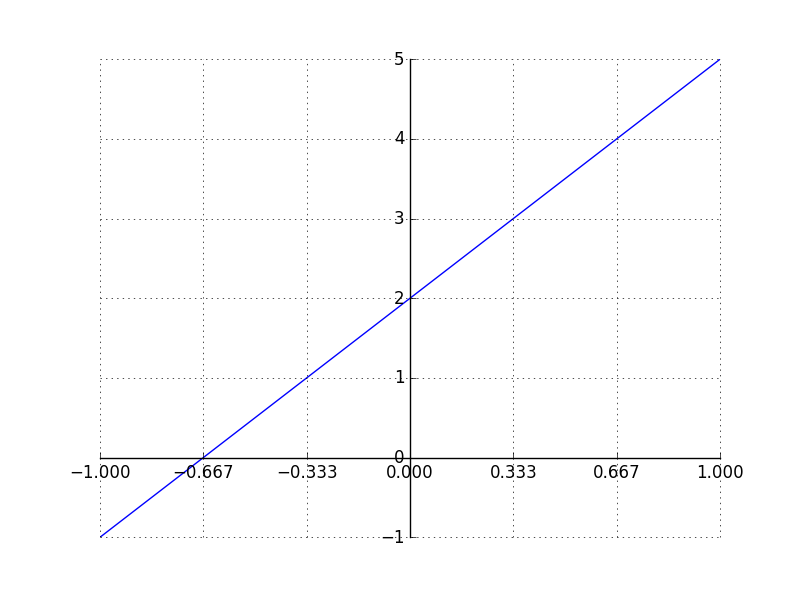
\includegraphics[scale = 0.5]{figures/3Xp2.png}
    \end{subfigure}%%
    \begin{subfigure}{.5\textwidth}
    \centering
    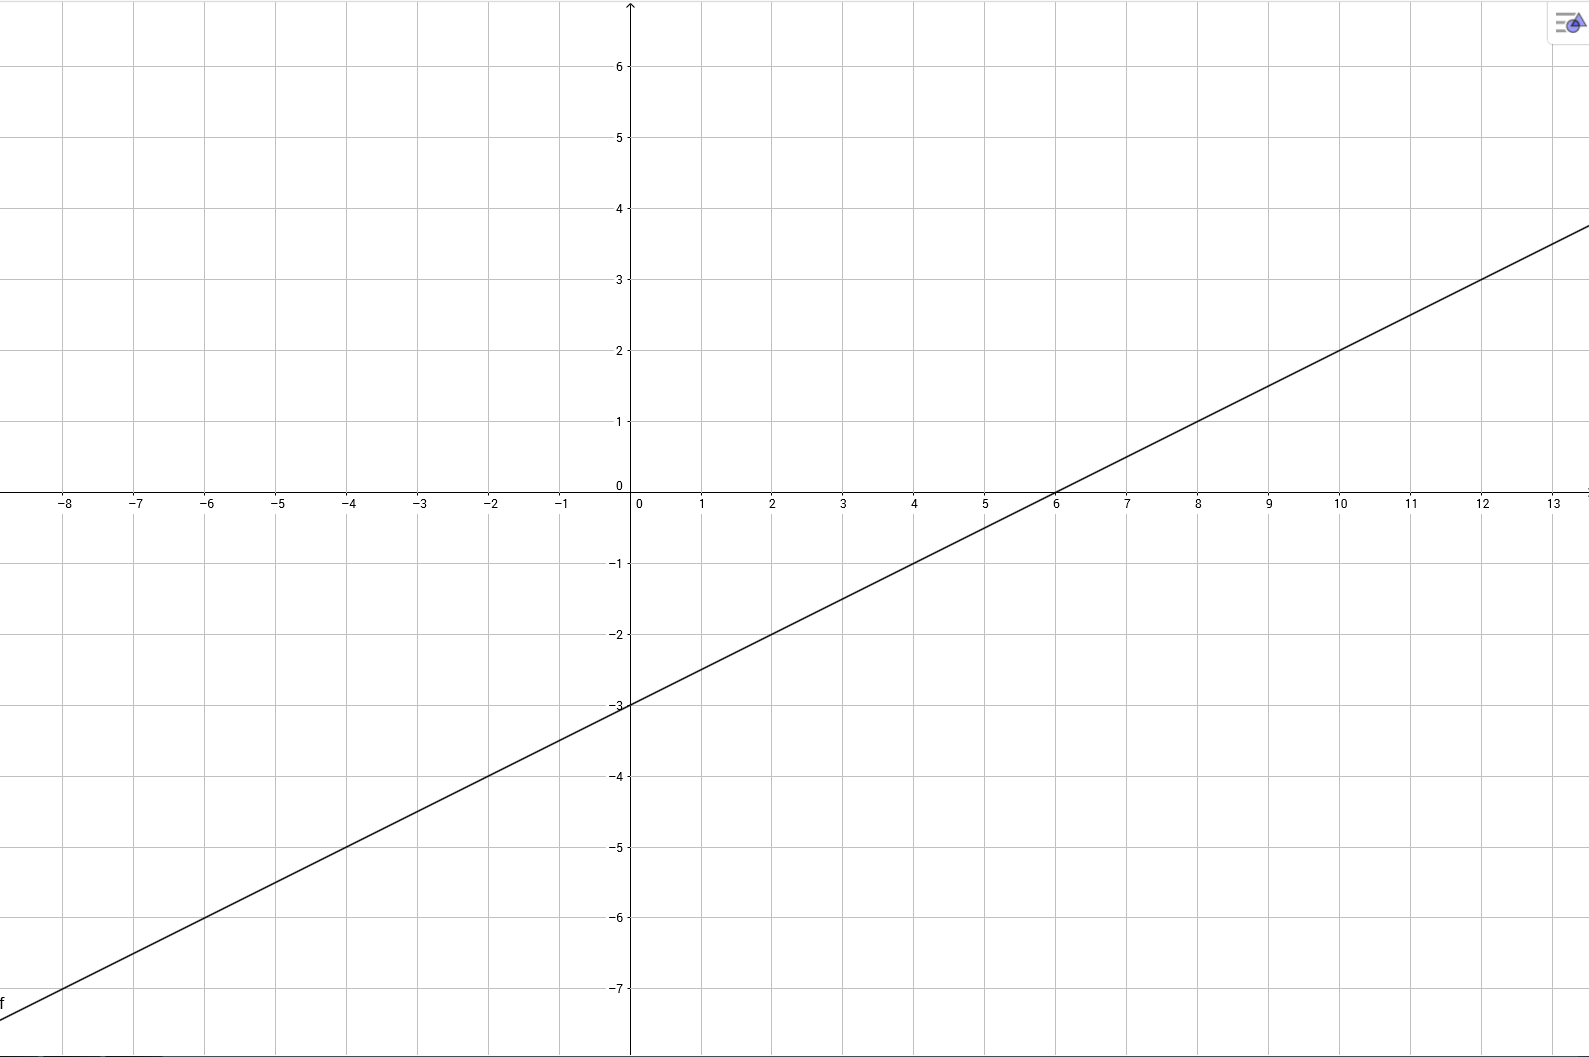
\includegraphics[scale = 0.5]{figures/05Xp2.png}
    \end{subfigure}
\end{figure}
{\color{Maroon}Hvis eleven forsatt ikke forstår vil da eleven presenteres med en video forklaring :  Video forklaring knappen dukker opp.}
\newline
\newline
\textbf{Video forklaring:}
\newline\newline
{\emph{\color{gray}
Husk at stigningstallet kan regnes ved å dele forandringen mellom y verdiene på forandringen i x-verdiene.}} 
\newline
{\color{PineGreen} På videoen vises formelen mens det forklares vha. grafen hvor oppleseren trekker en vertikal linje ned fra grafen fra en passelig funksonsverdi og deretter trekkes det en linje horisontalt inntil til funksjonen.} \newline\newline
{\emph{\color{gray}
Jeg kan velge passende $\Delta y$ og $\Delta x$ verdiene og sette disse inn i formelen for å regne ut stigningstallet.}} \newline
{\color{PineGreen} Det vises at oppleseren markerer $\Delta y$ og $\Delta x$ på grafen og skriver opp formelen.} 
\begin{figure}[h!]
\centering
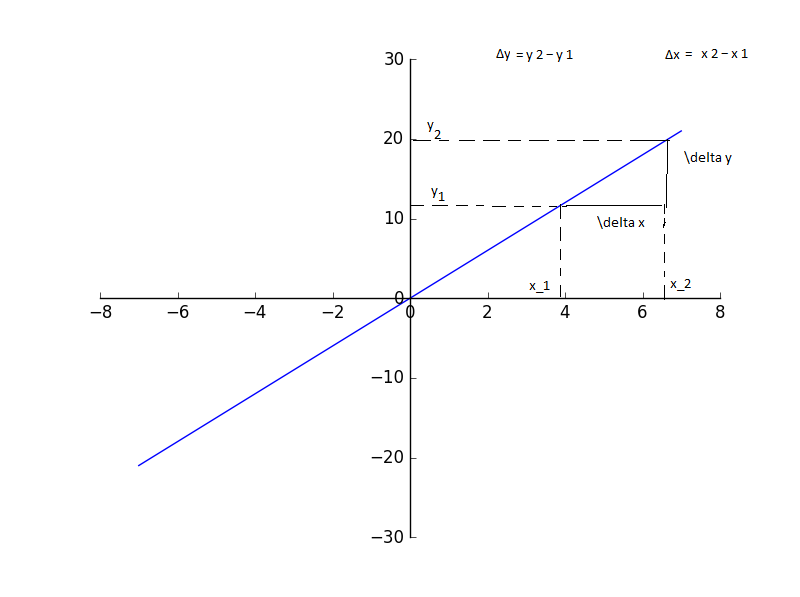
\includegraphics[scale = 0.6]{figures/stigningstallet.png}
\end{figure}
\newline\newline
{\emph{\color{gray}
F.eks i funksjonen $y = 3x$. Vi velger disse to punktene $y_2$ og $y_1$. Her ser vi at forandringen i y, er $\Delta y = y_2 - y_1 = 6- 0$ og forandringen i for disse funksjonsverdiene er $\Delta x_2 - \Delta x_1 = 2 - 0$. Da ser vi at stigningstallet blir $6/2 = 3.$}} \newline
{\color{PineGreen} Det vises at oppleseren gjentar avlesning fra funksjonen og markerer verdiene med striplet linje. Deretter setter oppleseren verdiene inn i formelen og regner ut stigningstallet.}
\begin{figure}[h!]
\centering
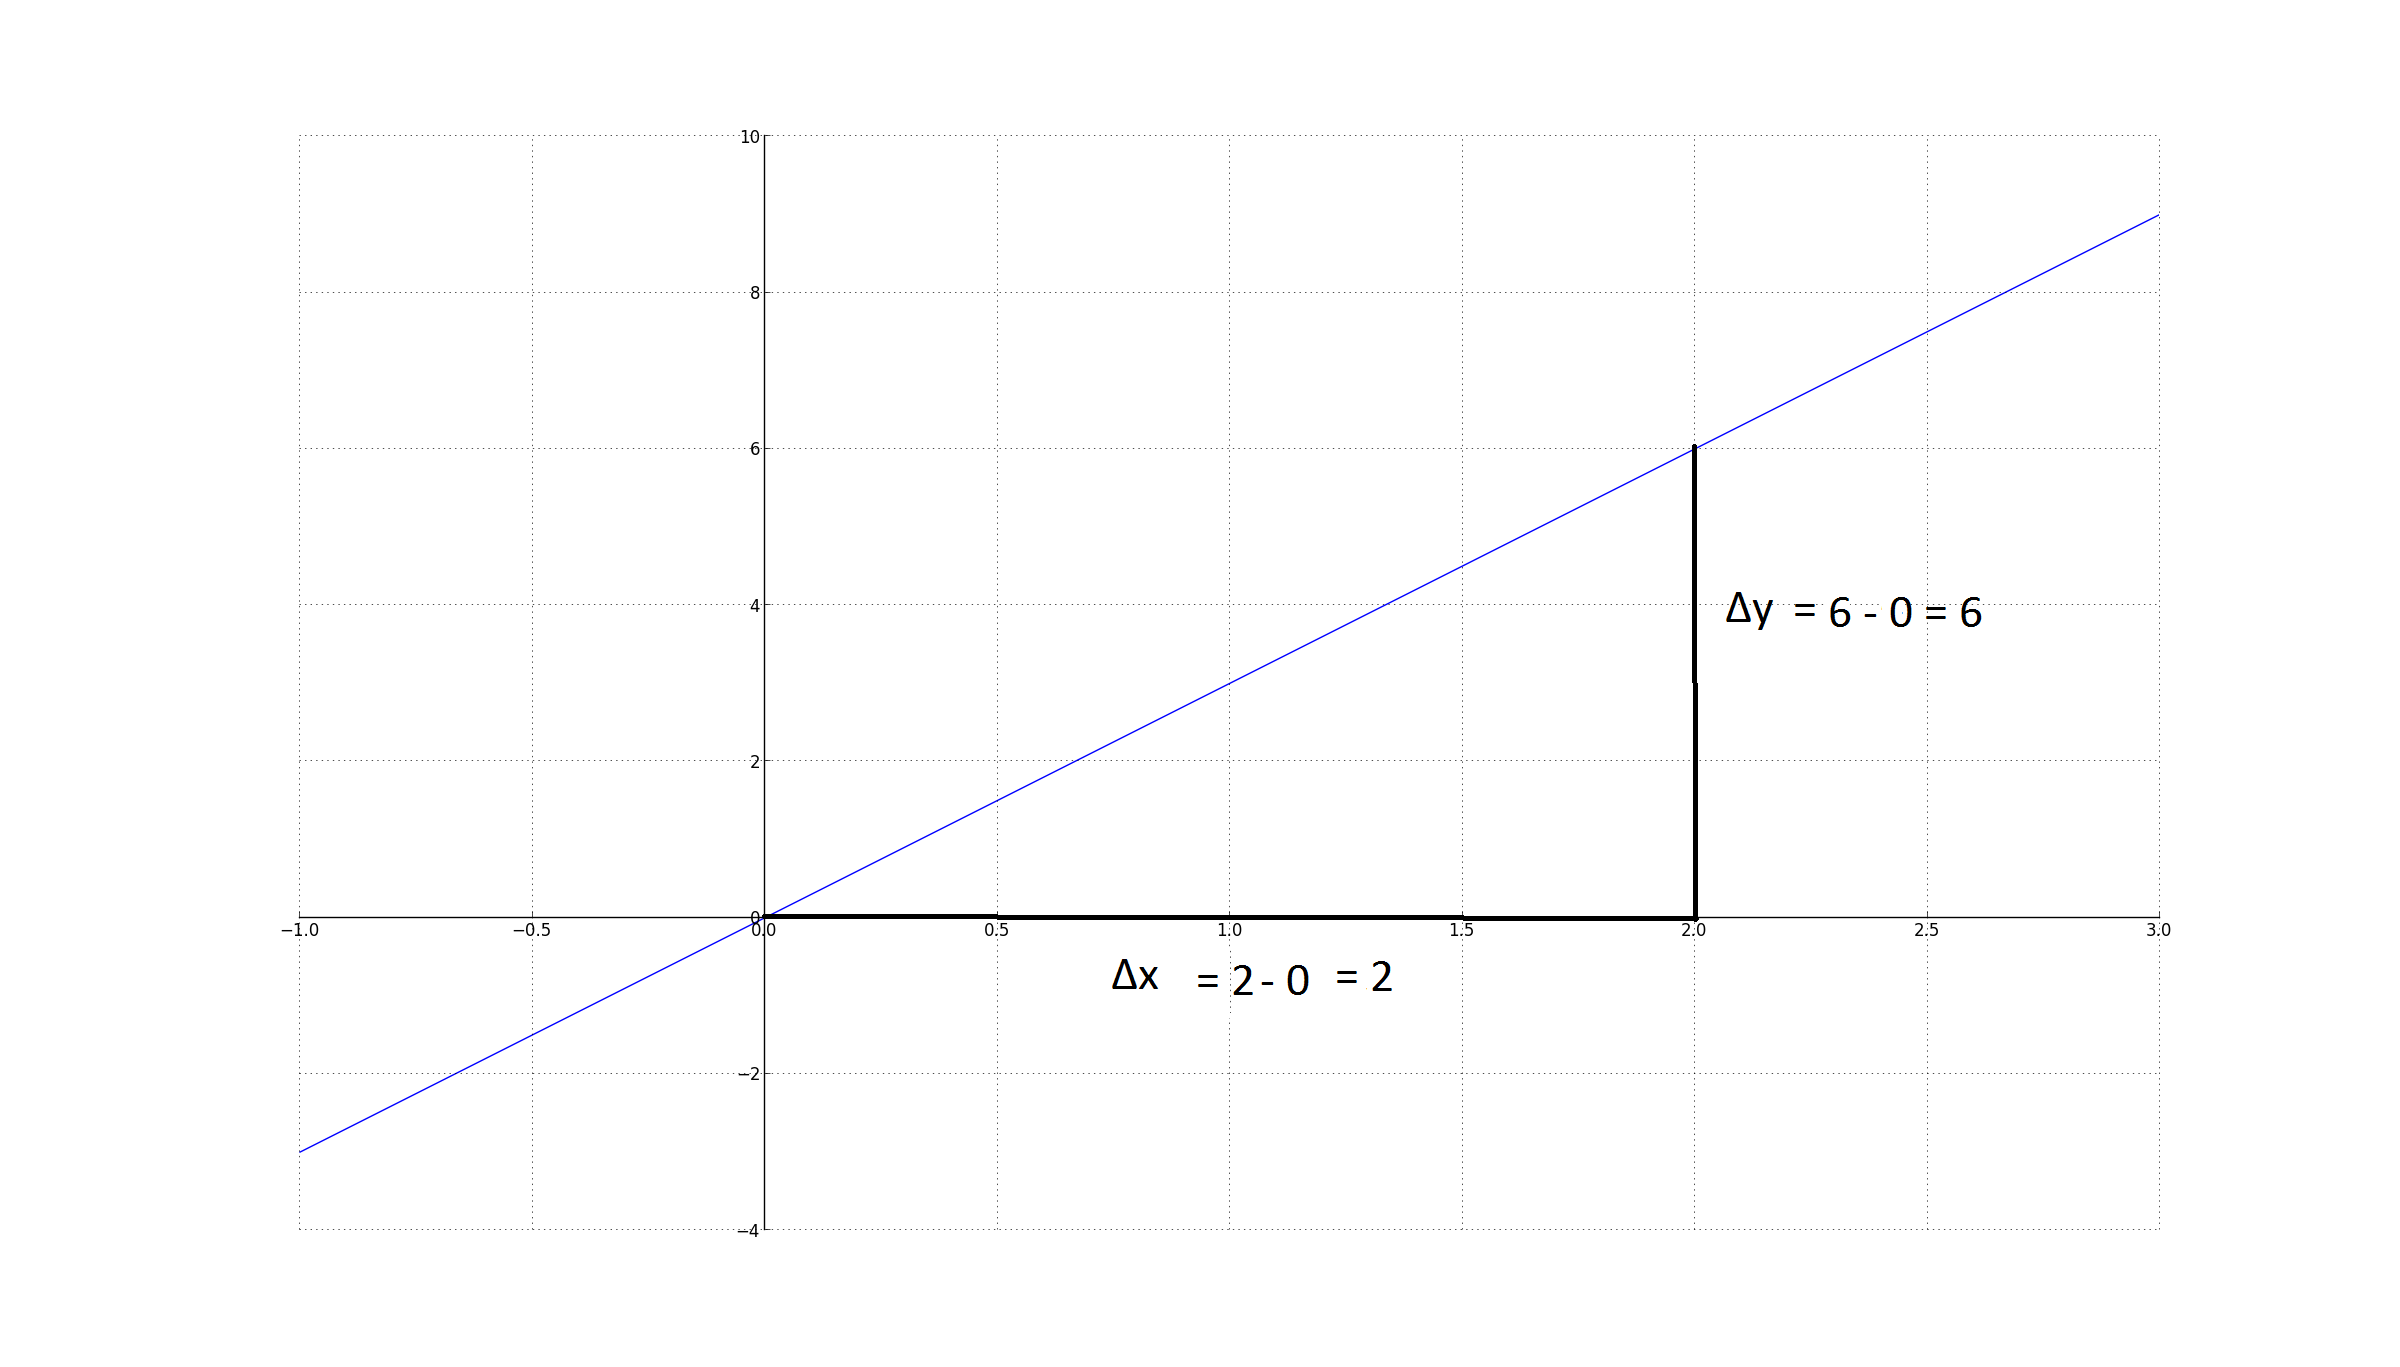
\includegraphics[scale = 0.3]{figures/stigningstalleksempelet.png}
\end{figure}
\end{Exercise}

\newpage
\newpage
\newpage
\subsection*{Konstantledd}

\begin{Exercise}
Finn verdien til y hvor funksjonen krysser y-aksen. (Tast verdien i svarfeltet) {\color{Cerulean} Hvordan bør svarfeltet brukes. Her skal svaret være en tall og da føler vi at det vanlige svarfeltet (se figuren under) blir for pregende.}
\begin{figure}[h!]
\centering
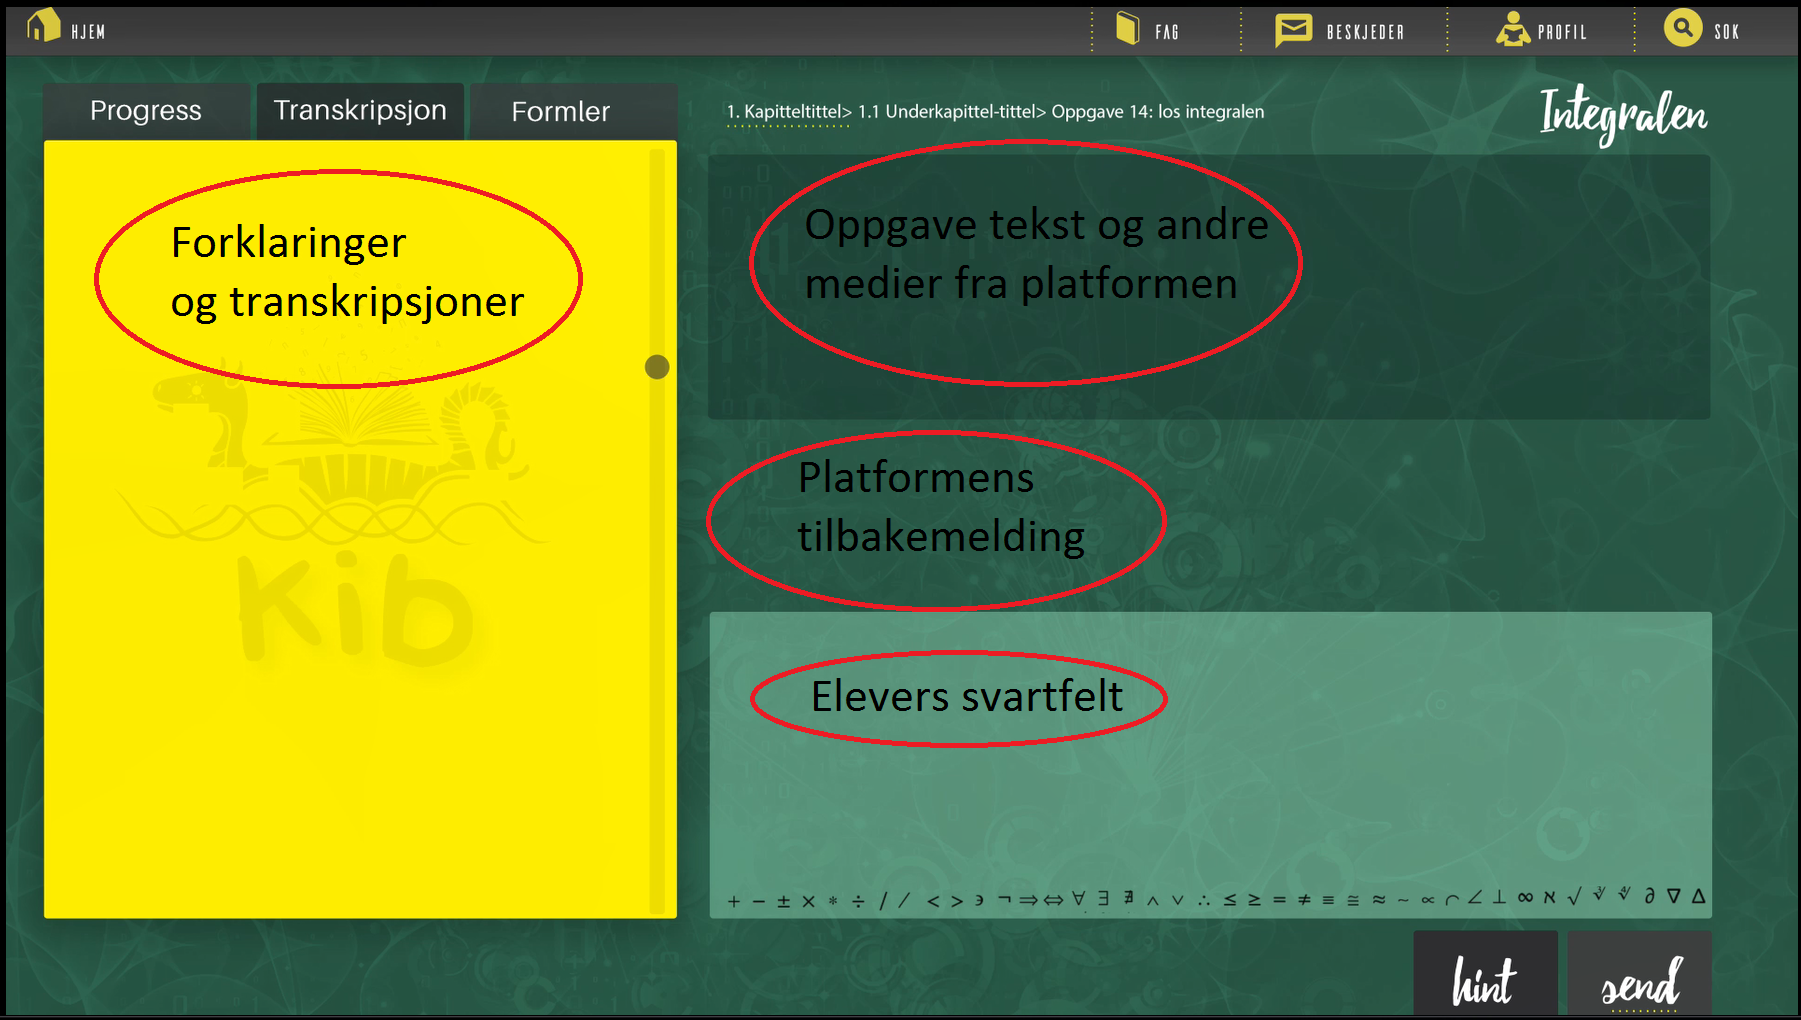
\includegraphics[scale = 0.3]{figures/Platform_explained.png}
\end{figure}
\end{Exercise}

\newpage
\begin{Exercise}
Finn konstantleddet til følgende lineære funksjoner. Fyll svaret i svarfeltet:
\begin{figure}[h!]
\centering
    \begin{subfigure}{.5\textwidth}
    \centering
    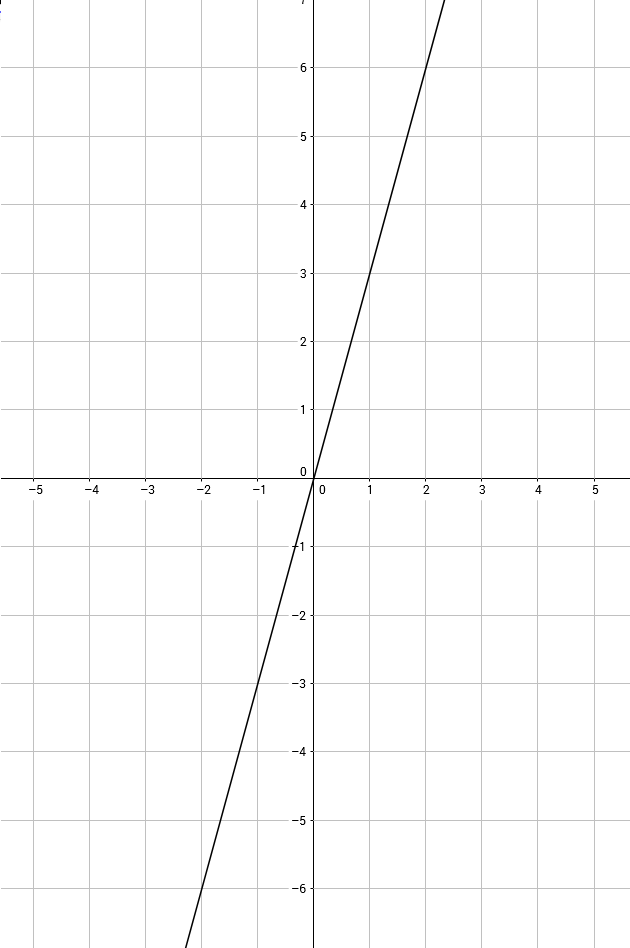
\includegraphics[scale = 0.5]{figures/3X.png}
    \end{subfigure}%%
    \begin{subfigure}{.5\textwidth}
    \centering
    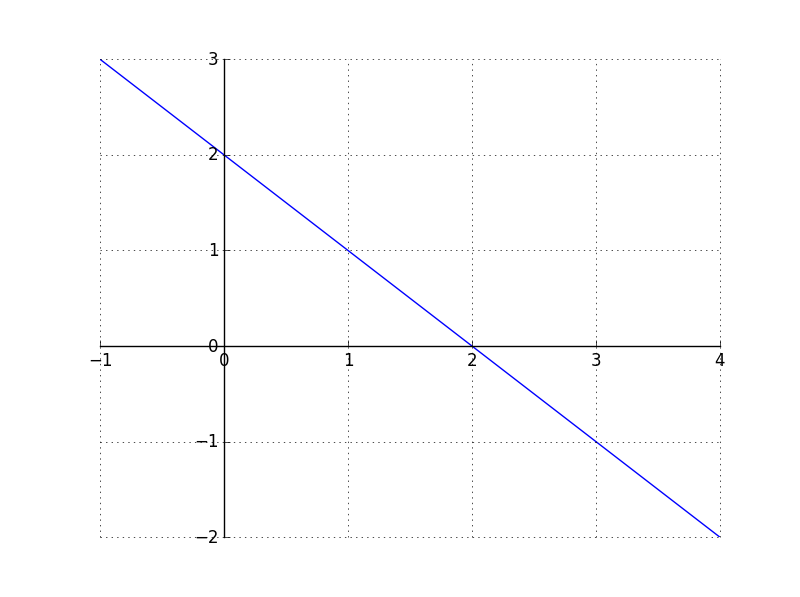
\includegraphics[scale = 0.5]{figures/mXp2.png}
    \end{subfigure}
    \begin{subfigure}{.5\textwidth}
    \centering
    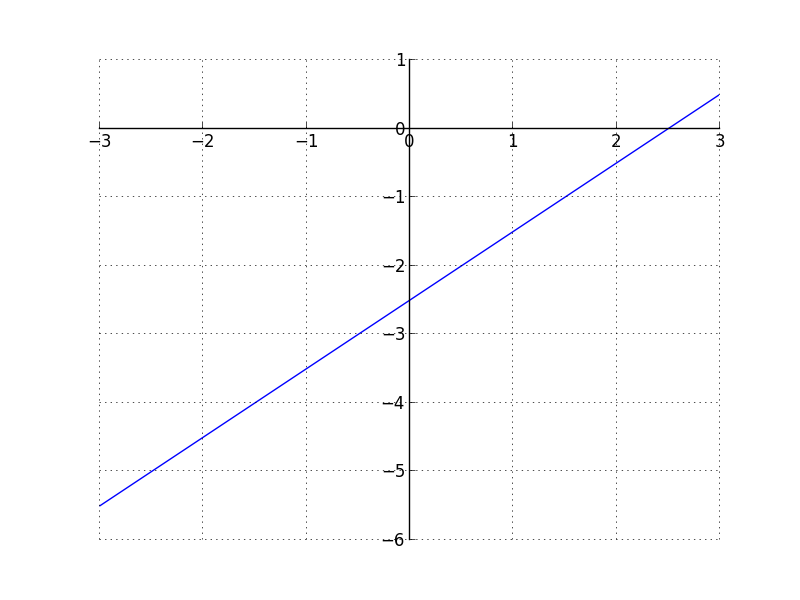
\includegraphics[scale = 0.5]{figures/Xm25.png}
    \end{subfigure}%%
    \begin{subfigure}{.5\textwidth}
    \centering
    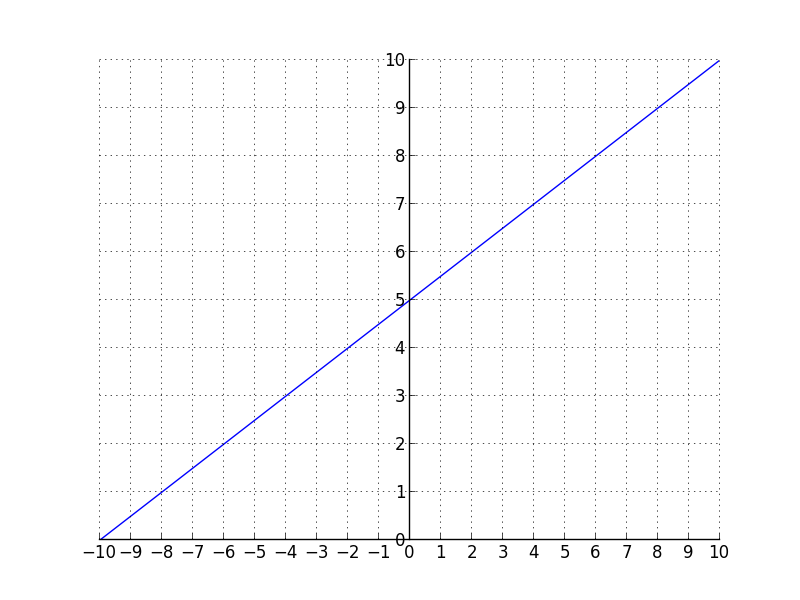
\includegraphics[scale = 0.5]{figures/05Xp5.png}
    \end{subfigure}
\end{figure}

{\color{Maroon}Hvis eleven taster feil:} \newline
{\color{gray}Husk at konstantleddet til funksjonen kan leses av figuren. Det er verdien til y der funksjonen krysser y-aksen.}
{\color{Maroon}Figur med utpekt verdi på funksjonen blir mens oppleseren forklarer eller tegner.}
\begin{figure}[h!]
\centering
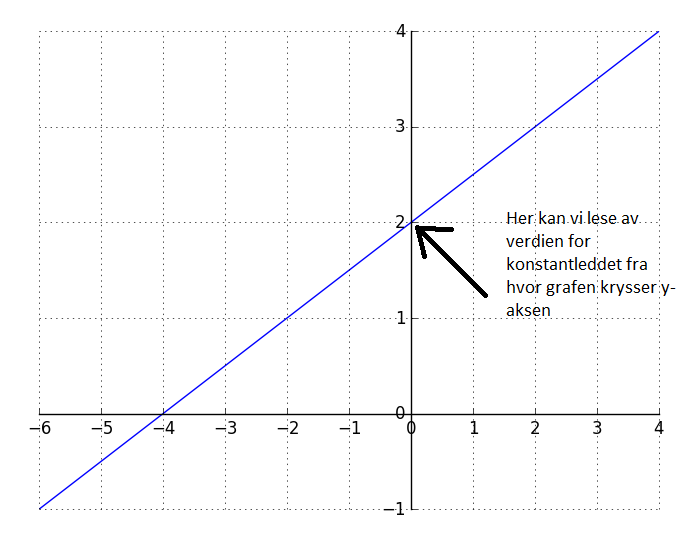
\includegraphics[scale = 0.4]{figures/konstantleddeksempelet.png}
\end{figure}
\end{Exercise}

\subsection*{Lineær funksjon}
I disse oppgavene  skal vi finne likninger til lineære funksjoner. Husk at en linje beskrives med likningen i formen $\mathbf{y} = {\color{blue}a}\mathbf{x}+ {\color{red}b}$ der ${\color{blue}a}$ er {\color{blue}stigningstallet} og ${\color{red}b}$ er \textbf{y} verdien ved krysnings punkt, dvs. {\color{red}konstantleddet}.

\begin{Exercise}
\textbf{Del 1)}
\newline
Skriv likning til linja som har stigningstallet $4$ og konstantledd $1$
\newline
\textbf{Svar}
\newline  
$y=4x+1$
\newline
\textbf{Hint 1}
\newline
Husk at likningen til en linje har formen $\mathbf{y} = {\color{blue}a}\mathbf{x}+ {\color{red}b}$ der ${\color{blue}a}$ er {\color{blue}stigningstallet} og ${\color{red}b}$ er {\color{red}konstantleddet}.
\newline
\textbf{Hint 2}
\newline
I dette tilfellet $a=4$ og $b=1$
\newline\newline
\textbf{Del 2)} 
\newline\newline
Hvilken graf tilhører denne funksjonen? 
\newline
{\color{Maroon}Det skal vises følgende funksjoner:
\newline
$y=4x+1$
\newline
$y=4x+5$
\newline
$y=1x+4$
\newline
$y=5x+3$
}
\begin{figure}[h!]
\centering
    \begin{subfigure}{.5\textwidth}
    \centering
    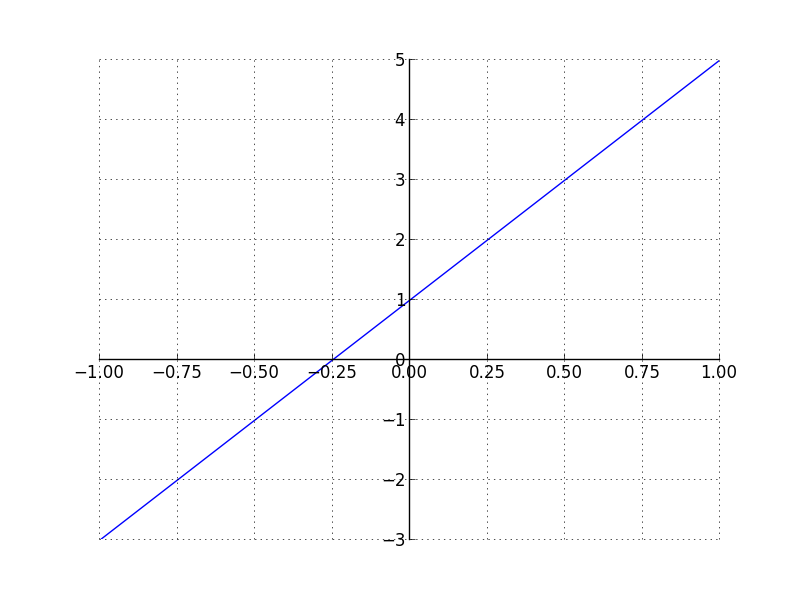
\includegraphics[scale = 0.5]{figures/4Xp1.png}
    \end{subfigure}%%
    \begin{subfigure}{.5\textwidth}
    \centering
    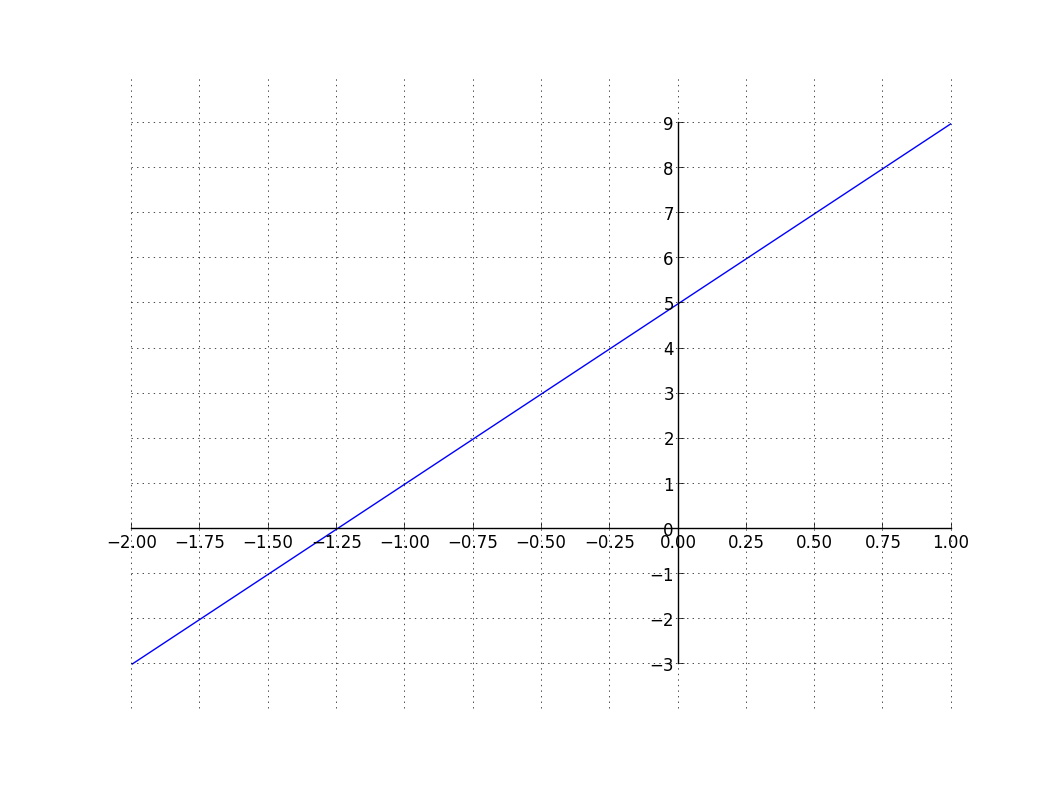
\includegraphics[scale = 0.4]{figures/4Xp5.png}
    \end{subfigure}
    \begin{subfigure}{.5\textwidth}
    \centering
    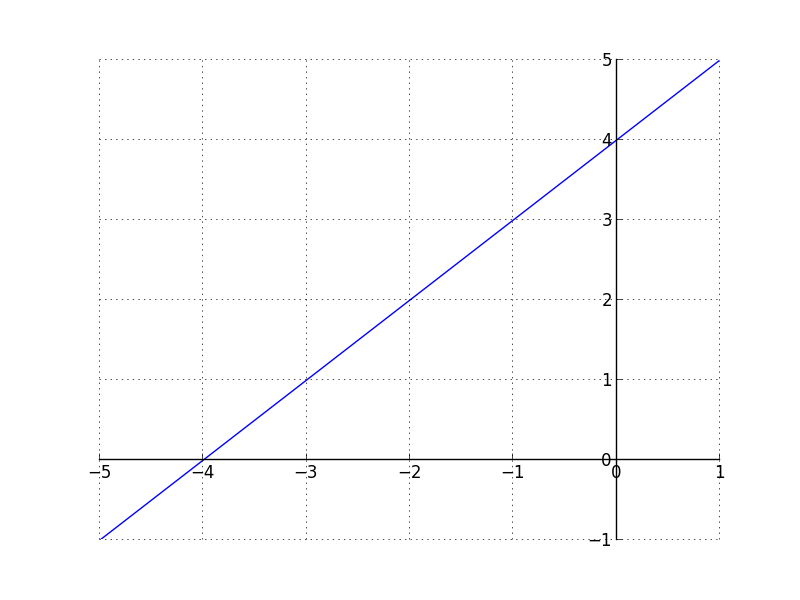
\includegraphics[scale = 0.5]{figures/Xp4.png}
    \end{subfigure}%%
    \begin{subfigure}{.5\textwidth}
    \centering
    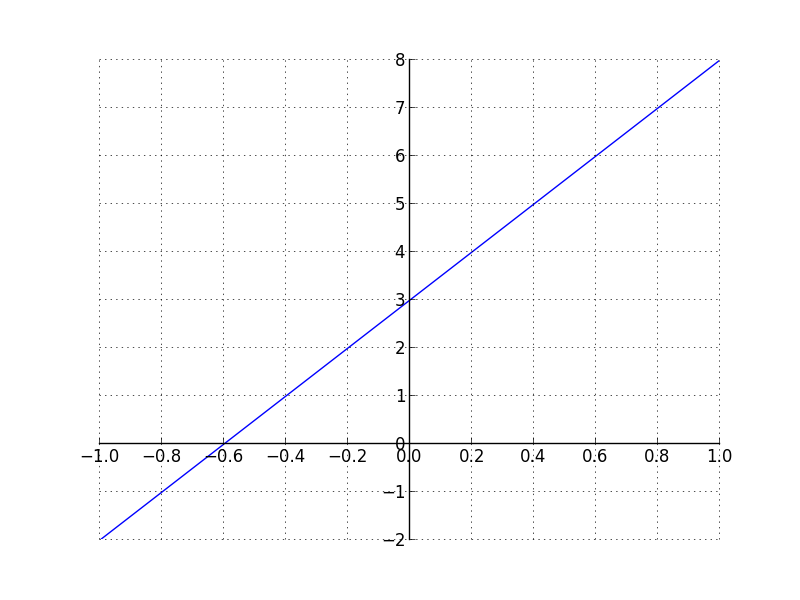
\includegraphics[scale = 0.5]{figures/5Xp3.png}
    \end{subfigure}
\end{figure}
\end{Exercise}

\begin{Exercise}
Skriv likning til linja som har stigningstallet $-2$ og som krysser y aksen på $3$
\newline\newline
\textbf{svar}  
\newline
$y=4x+1$
\newline
\textbf{Hint 1}
\newline
Husk at likningen til en linje har formen $y=ax+b$ der $a$ er stigningstallet og $b$ er y verdien ved krysnings punkt.
\newline
\textbf{Hint 2}
\newline
I dette tilfellet $a=-2$ og $b=3$
\newline\newline
\textbf{Oppgave 1.b} Hvilken graf tilhører denne funksjon? 
\newline
{\color{Maroon}Det skal vises følgende funksjoner:
\newline
$y=-2x+3$
\newline
$y=2x+-3$
\newline
$y=-3x+2$
\newline
$y=-3x+3$
}
\end{Exercise}

\begin{Exercise}
Skriv likningen som beskriver linear funksjon som vises i denne grafen:
\newline
{\color{Maroon} The graph will show this linear function: $y = 6x-3$:}
\newline
\newline
\textbf{Hint 1}
\newline
Husk at likningen til en linje har formen $y=ax+b$ der $a$ er stigningstallet og $b$ er y verdien ved krysnings punkt.
Hva er stigningstallet til denne linearfunskjon? 
$a=$
Hvor krysser funksjonen y aksen? 
$b=$
\end{Exercise}


%%%%%%%%%%%%%%%%%%%%%%%%%%%%%%%%%%%%%%%%%%%%%%%%%%%%%%%%%%%%%%%%%%%%%
%%%%%%%%%%%%%%%%%%%% Oppgave 13    %%%%%%%%%%%%%%%%%%%%%%%%%%%%%%%%%%
%%%%%%%%%%%%%%%%%%%%%%%%%%%%%%%%%%%%%%%%%%%%%%%%%%%%%%%%%%%%%%%%%%%%%
\begin{Exercise}
\hspace{-6.5mm}Finn likning til linja som går gjenomm punktene $(2,6)$  og  $(0,-4)$
\newline\newline
{\color{Maroon} Det skal vises en knapp hvor det står løsningsforslag. Dersom elev trykker på løsningsforlag knappen kommer vil løsningsforslag rammen ta større plass og alle skrittene vil bli synlige.} 
\newline
\newline
\newline
\st{\textbf{Hint }}
\newline
\textbf{Løsningsforslag :}
\newline
{\color{Maroon}Først gir plattformen en oversikt over hva skal skje: Dette vil forekomme i løsningsforslag rammen} 
\newline
{\color{Cerulean} Følgende tekst med ligningen bør legges både i svarfeltet til eleven og i løsningsforslag rammen}
\newline
\textbf{Likning til ei linje er gitt på denne formen:}
\begin{align}
y=\mathbf{a}x + \mathbf{b}
\end{align}
Det vil si at vi vil finne stigninstallet $\mathbf{a}$ og konstantleddet $\mathbf{b}$ slik at de gitte punktene befinner seg på den rette linja. Dette skal vi gjøre i 4 skritt.
\newline
\newline
{\color{Cerulean} Fire skritt vil være synlige i løsningsforslag rammen. Innhold til hver skritt vil være skjult før bruker ber om innhold}
\newline
\begin{enumerate}
%%%%%%%%%%%%%%%%%%%%%%%%%%%%%     SKRITT 1      %%%%%%%%%%%%%%%%%%%%%%%%%%%%%%%%%%%%%%
\item Først \st{kan vi finne} finner vi stigninstallet $\mathbf{a}$  ved å bruke formelen:

\begin{align}
a =  \frac{y_2 - y_1}{x_2 - x_1}
\end{align}
med de gitte punktene
$
\begin{matrix}
  x_1\:\:\: y_1 \\ 
 (0,\:-4) \\
\phantom{0}
\end{matrix}
$ og $
\begin{matrix}
  x_2\:\:\: y_2 \\ 
 (2,\:\:\:6)  \\
\phantom{0}
\end{matrix}
$ 
\newline
\textbf{Finn $\mathbf{a}$ ved å sette verdiene til punktene i svarfeltet.}
\newline
\newline
{\color{Maroon} Det oppstår $a=\frac{\square-\square}{\square-\square}$ på svarefeltet. Bruker vil ha muligheten til å finne hver rubrikk med tall og senere ha muligheten til å forkorte brøken. Hvis brukeren klarer ikke å fylle riktig tall selv oppstår det en knapp til  forklaringsvideo, men det er ikke nødvendig at alle elever ser på det. Videon skal bare vises  dersom de trykker på knappen.}
\newline
\newline
{\color{gray} La oss finne stigningstallet ved å bruke formelen a er lik forandring på y delt på forandring på x } \newline
{\color{PineGreen} The equation for the slope is written: $a =  \frac{y_2 - y_1}{x_2 - x_1}$ } \newline
{\color{gray}  For å finne forandring på y,tar vi differansen i y koordinatene, som i dette tillfelle er 6 minus minus 4 } \newline
{\color{PineGreen}  6 -(- 4) is inserted in the nominator of the formula} \newline
{\color{gray}  For å finne forandring på x,tar vi differansen i x koordinatene, som i dette tillfelle er 2 minus 0 } \newline
{\color{PineGreen} 2 - 0 is inserted in the denominator of the formula  } \newline
{\color{Maroon}  Etter videoen må brukeren selv sette inn tallene.}

%%%%%%%%%%%%%%%%%%%%%%%%%%%%%%%%%%    SKRITT 2    %%%%%%%%%%%%%%%%%%%%%%%%%%%%%%%%%%%%%%%%%%%%%%%%%%%
\item Sett inn verdien vi har funnet for stigningstallet i den opprinelige likgningen: $y = ax + b$ 
\newline
\textbf{Sett opp likningen: $y = ax + b$ med verdien for stigningstallet.}
\newline
{\color{Maroon} Hvis brukeren klarer ikke å fylle riktig tall selv, oppstår det formel i svarfeltet med blanktegn: 
\begin{align}
y = \underline{\phantom{0}}x + b
\end{align}}
{\color{Maroon}  Hvis brukeren klarer ikke å fylle riktig tall selv oppstår det igjen en knapp til  forklaringsvideo, men igjen det er ikke nødvendig at alle elever ser på det. Videon skal bare vises  dersom de trykker på knappen.}
\newline
\newline
{\color{gray} Nå at vi har funnet stigningstallet kan vi sette den i formelen  $y = ax + b$ } \newline
{\color{PineGreen} $y = ax + b$  } \newline
{\color{gray}Vi erstatter "a" med tall verdien 5 } \newline
{\color{PineGreen} the letter a is erased and replaced with the number 5 }

%%%%%%%%%%%%%%%%%%%%%%%%%%%%%%%%%%    SKRITT 3    %%%%%%%%%%%%%%%%%%%%%%%%%%%%%%%%%%%%%%%%%%%%%%%%%%%
\item Nå må vi finne konstantleddet b. \st{, for} For å gjøre det velger vi et punkt og ersatter koordinatene i ligningen $y_1=5x_1+b$ og deretter løser vi ligningen for b. 
\newline
\textbf{Velg et punkt og erstatt $\mathbf{x}$ og $\mathbf{y}$ i likningen $y=5x+b$ og løs uttrykket for b.}
\newline
{\color{Maroon} Det skal oppstå en hintknapp og en videoforklaringsknapp. Dersom eleven trykker på hintknappen oppstår det følgende i løsningsforslagsrammen}
\newline
\newline
%%%%%%%%%%%%%%%%%%%%%%     HINT 1      %%%%%%%%%%%%%%%%%%%%%%%%%%%%%
\textbf{Hint 1}
\newline
Sett inn $x_1$ og $y_1$ verdiene fra et av punktene og løs for b.
\newline
{\color{Maroon} Følgende oppstår samtidig (når elev trykker på hint-knappen) i svarfeltet}
\begin{align}
\square = 5\cdot\square + b
\end{align}
{\color{Maroon} Dersom elev ber om ytterligere hint, kan eleven trykke på neste hint knapp.}
\newline
\newline
%%%%%%%%%%%%%%%%%%%%%%     HINT 2      %%%%%%%%%%%%%%%%%%%%%%%%%%%%%
\textbf{Hint 2}
\newline
Ved å foreksempel velge punktet $(0,-4)$ kan det settes inn i likningen.
\newline
\textbf{ Løs for b}
\begin{align}
(\, -4 \, ) = 5\cdot (\, 0 \, ) + b \\
\end{align}
{\color{gray}For å  finne konstantleddet b  velger vi et punkt og ersatter koordinatene i ligningen. For eksempel velger jeg (2,6). Så jeg skal erstatte 6 med y og 2 med x} \newline
{\color{PineGreen} write down the two points  $(2,6)$  and  $(0,-4 )$ above the equation and draw a red circle around $(2,6)$ . Then draw an arrow coming from 6 to y and another from 2 to x (see figure \ref{fig:Opp11S4})}
\begin{figure}[h!]
\label{fig:Opp11S4}
\centering
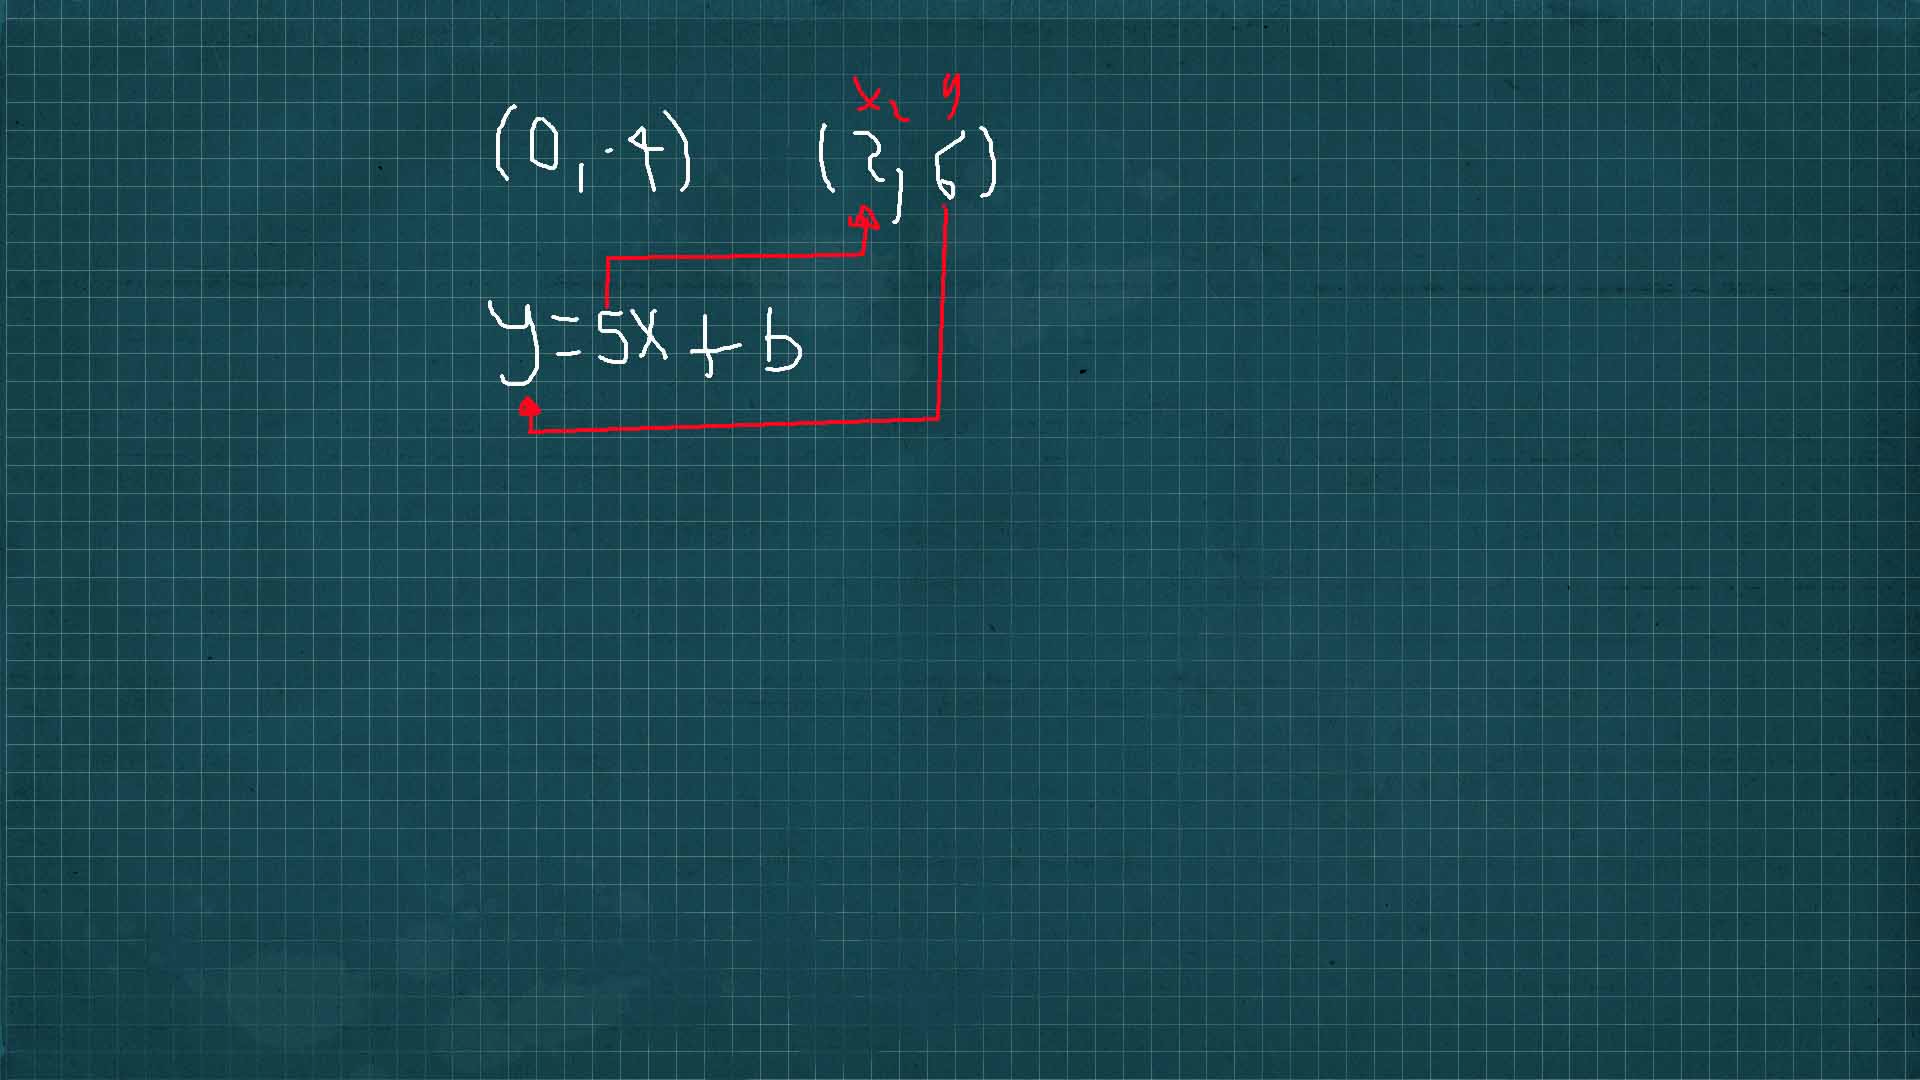
\includegraphics[scale = 1.3]{figures/Opp11S4.jpg}
\end{figure}
{\color{gray} Vi får da ligningen $6=5\cdot 2+b$, der b er en unkjent} \newline
{\color{PineGreen} write down equation 
\newline
$6=5\cdot 2+b$}
\newline
{\color{gray} Vi løser for b og får at b er lik $6-10$ som er lik -4}
\newline
{\color{PineGreen} write down equation
\begin{align}
b=6-10=-4
\end{align}}

%%%%%%%%%%%%%%%%%%%%%%%%%%%%%%%%%%    SKRITT 4    %%%%%%%%%%%%%%%%%%%%%%%%%%%%%%%%%%%%%%%%%%%%%%%%%%%
\item Siste skritt for å svare på oppgaven er å skrive opp utrrykket for funksjonen ved å sette verdiene vi har funnet for stignnigstallet og konstanleddet.
\newline
Sett disse verdiene i likningen.
\newline
{\color{Maroon} Hvis brukerer vet ikke hva han skal gjøre får han \mbox{hint :}} 
\newline
\newline
\textbf{Hint:}
\begin{align}
y = \square x + \square
\end{align}
{\color{Maroon} Hvis brukerer forsatt vet ikke hva han skal gjøre kan han trykke på neste hint-knappen:}
\newline
\newline
\textbf{Hint:}
\begin{align}
  &\,\,\quad a \qquad b\\ 
y &= \square x + \square\\
\end{align}
\end{enumerate}
{\color{gray}For å fullføre oppgave erstatter vi verdiene vi har funnet for a og b i linearlikningen. Så vi for at $y=5x-4$}
\newline
{\color{PineGreen} When he says "a" we write $a=5$ and when he says "b" we write $b=-4$, then below we write $y=5x-4$} 
\newline
\newline
%%%%%%%%%%%%%%%%%%%%%%%%%% OPPSUMMERING  %%%%%%%%%%%%%%%%%%%%%%%%%%%%%%%%%%%%%
{\color{Maroon}Tilslutt skal det gis følgende oppsummering :}
\begin{itemize}
\item Finn først stigningstallet ved å bruke formelen :
\begin{align}
a =  \frac{y_2 - y_1}{x_2 - x_1}
\end{align}
\item Sett inn stigningstalllet i funksjonen og løs ligning for konstantleddet b:
\begin{itemize}
\item Sett opp et uttrykk for ligningen hvor b er ukjent :
\begin{align}
b = y_1 - a\cdot x_1
\end{align}
\item Velg et punkt $(x_1, y_1)$ og sett den inn for uttrykket for b
\end{itemize}
\item Tilslutt skal uttrykket for ligningen settes opp ved innsetting av stigningstallet og \mbox{konstantledet:}
\begin{align}
y = ax + b.
\end{align}
\end{itemize}
\end{Exercise}



%%%%%%%%%%%%%%%%%%%%%%%%%%%%%%%%%%%%%%%%%%%%%%%%%%%%%%%%%%%%%%%%%%%%%%%%%
%%%%%%%%%%%%%%%%%%%%%%%%% Oppgave 14 %%%%%%%%%%%%%%%%%%%%%%%%%%%%%%%%%%%%
%%%%%%%%%%%%%%%%%%%%%%%%%%%%%%%%%%%%%%%%%%%%%%%%%%%%%%%%%%%%%%%%%%%%%%%%%
\begin{Exercise}
\label{ex:12}
Finn funksjonen som er parallel med $y = 5x - 4$.
\newline
\begin{figure}[h!]
    \centering
    \begin{subfigure}{.5\textwidth}
    \centering
    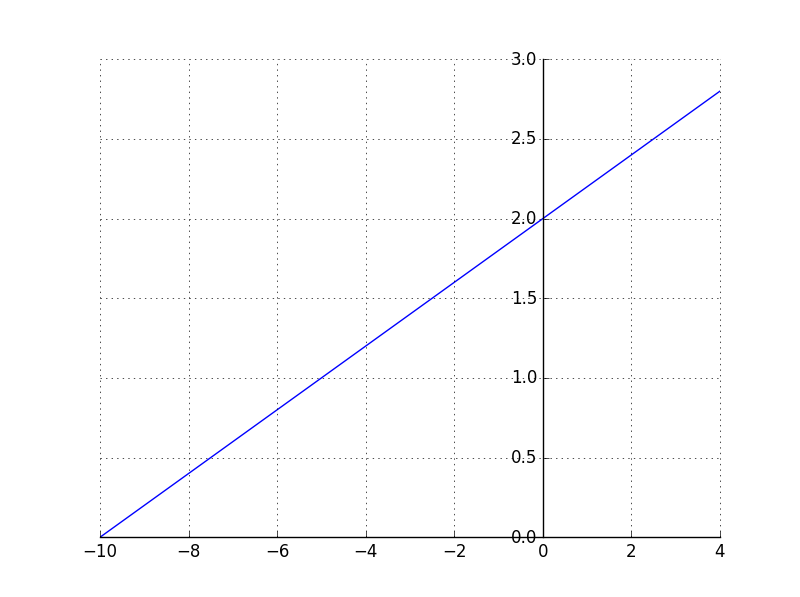
\includegraphics[scale = 0.4]{figures/xd5p2.png}
    \end{subfigure}%%
    \begin{subfigure}{.5\textwidth}
    \centering
    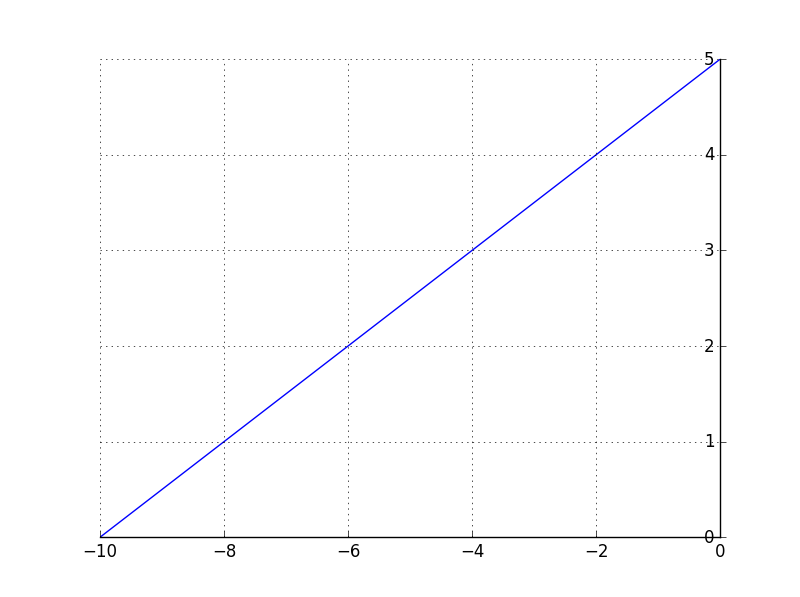
\includegraphics[scale = 0.4]{figures/xd2p5.png}
    \end{subfigure}
    \begin{subfigure}{.5\textwidth}
    \centering
    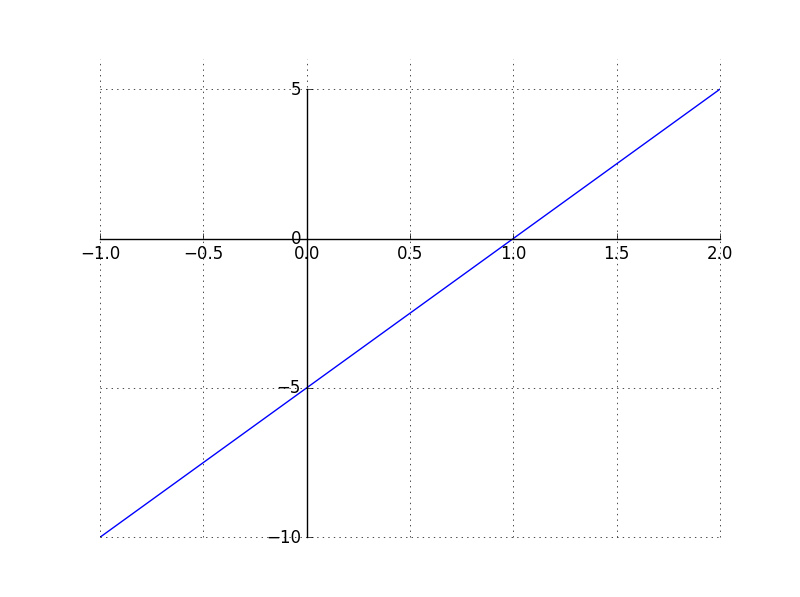
\includegraphics[scale = 0.4]{figures/5xm5.png}
    \end{subfigure}
    \caption{Figurer til oppgave \ref{ex:12}}
\end{figure}
{\color{Cerulean} Hvordan kan figurene trykkes og bruker bli opplyst om svaret var riktig eller feil?}
\newline
\newline
{\color{Maroon} Hvis brukerer velger feil funksjon.}
\newline
\textbf{Hint:} En funksjon er parallel med en annen funksjon hvis de har samme stigningstall. 
\newline
\newline
{\color{Maroon} Hvis brukerer trenger ytterlig hint}
\newline
\textbf{Hint:} Stigningstallet kan finnes ved å bruke følgende formel :
\begin{align}
a = \frac{y_2 - y_1}{x_2 - x_1}
\end{align} 
\newline
\newline
\textbf{Hint:} Velg to punkter fra figurene og regn ut stiningstallet. 
\newline
\newline
\textbf{Hint:} Sammenlign stiningstallet du har regnet med den til funksjonen $y = 5x - 4$.
\newline
\newline
{\color{Maroon} Hvis brukerer velger å få et løsningsforslag, vil følgende vises i plattformen.}
%%%%%%%%%%%%%%%%%% Løsningsforslag %%%%%%%%%%%%%%%%%%
\begin{enumerate}
\item Vi må først finne stigningstallet til hver figur og sammenligne verdien vi får med stiningstallet til den oppgitte funksjonen: $y = 5x - 4$. 
\begin{figure}[h!]
    \label{fig:xd5p2}
    \centering
    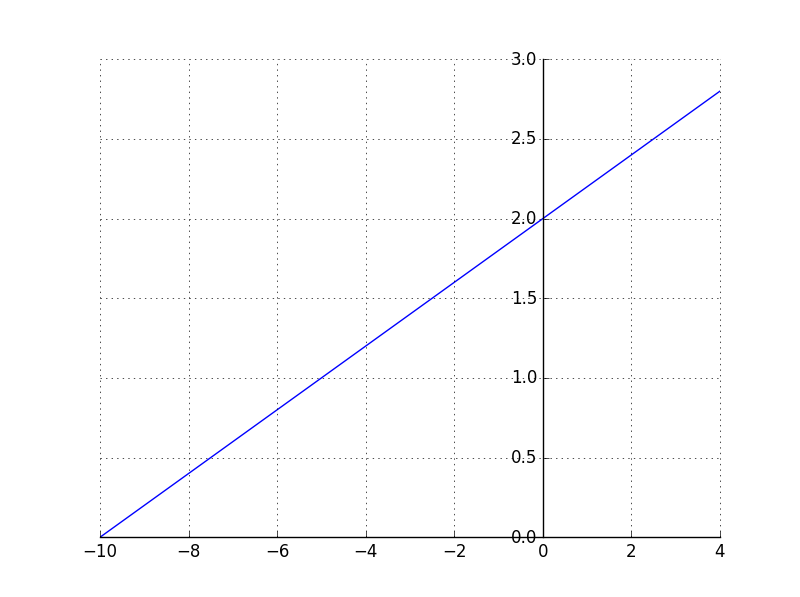
\includegraphics[scale = 0.4]{figures/xd5p2.png}
\end{figure}
\item La oss begynne med figur \ref{fig:xd5p2}. Vi leser av figuren to punkter, f.eks: $(-10,0)$ og  $(0,2)$.
\item Vi regner ut stiningstallet som er gitt ved følgende formel: 
\begin{align}
a = \frac{y_2 - y_1}{x_2 - x_1}
\end{align} 
Ved å sette inn tallene, får vi at
\begin{align}
a &= \frac{y_2 - y_1}{x_2 - x_1} = \frac{2 - 0}{0 - (-10)}\\
  &= \frac{1}{5}
\end{align} 
\item For å bekrefte om stigningstallet samsvarer med stigningstallet til funksjonen $y = 5x - 4$ må vi finne a verdien til denne funksjonen. Ved å huske at formelen for en generell lineær funksjon er gitt ved $y = ax + b$ ser vi at vi kan lese av verdien fra funksjonen for a, som blir da 5. Dermed kan vi se at figur \ref{fig:xd5p2} har ikke samme stiningstall og er derfor ikke parallel med $y = 5x - 4$.
\item Vi gjentar denne prosessen for de foregående funksjoner. 
\end{enumerate}
\end{Exercise}

\end{document}
